%%%%%%%%%%%%%%%%%%%%%%%%%%%%%%%%%%%%%%%%%%%%%%%%%%%%%%%%%%%%%%%%%%%%%%%%%%%%%%%%%%
\begin{frame}[fragile]\frametitle{}
\begin{center}
{\Large Theory: How it works?}
\end{center}
\end{frame}


%%%%%%%%%%%%%%%%%%%%%%%%%%%%%%%%%%%%%%%%%%%%%%%%%%%%%%%%%%%%%%%%%%%%%%%%%%%%%%%%%%
\begin{frame}[fragile]\frametitle{How Mind and Memory Work}
    \begin{columns}
        \begin{column}{0.48\textwidth}
			\begin{itemize}
				\item In typical awake states:
					\begin{itemize}
						\item Sense organs send signals to the conscious mind.
						\item Conscious mind decides what information to relay to the brain.
						\item The brain processes, references memories, and creates responses or stores knowledge.
					\end{itemize}
				\item In sleep:
					\begin{itemize}
						\item Only critical or threatening signals are relayed.
						\item Subconscious mind remains active, processing memories without conscious interference.
					\end{itemize}
			\end{itemize}
        \end{column}
        \begin{column}{0.48\textwidth}	
			  \begin{center}
				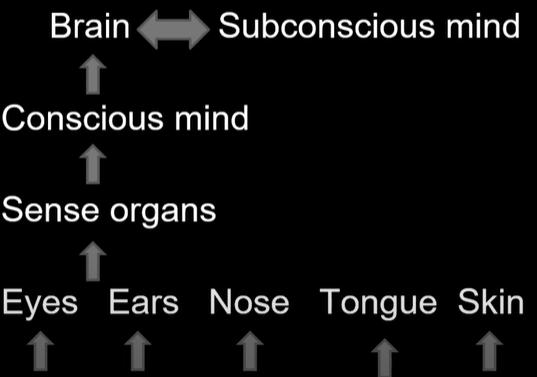
\includegraphics[width=\linewidth,keepaspectratio]{yoganidra14}

				{\tiny (Ref: Yoga Nidra as Therapy - Yogapointindia)}		
				\end{center}	
        \end{column}
    \end{columns}				
\end{frame}

%%%%%%%%%%%%%%%%%%%%%%%%%%%%%%%%%%%%%%%%%%%%%%%%%%%%%%%%%%%%%%%%%%%%%%%%%%%%%%%%%%
\begin{frame}[fragile]\frametitle{Changes in Yoganidra: Bypassing the Brain}

    \begin{columns}
        \begin{column}{0.48\textwidth}
			\begin{itemize}
				\item In Yoganidra:
					\begin{itemize}
						\item The conscious mind bypasses usual processes, directly influencing the subconscious.
						\item Desired affirmations or resolutions can overwrite or reprogram unwanted memories.
						\item This bypass allows deeper, lasting personal transformation without mental resistance.
					\end{itemize}
				\item Conscious instructions integrate seamlessly into the subconscious, enabling habit or perception changes.
			\end{itemize}
        \end{column}
        \begin{column}{0.48\textwidth}	
			  \begin{center}
				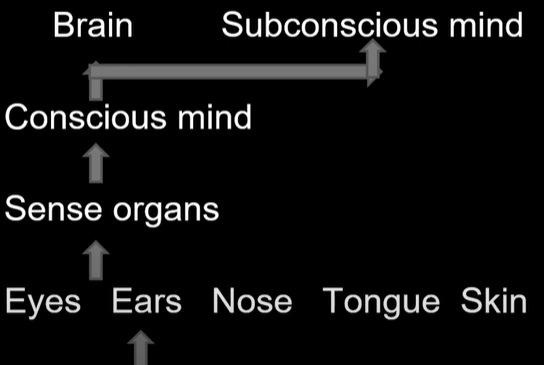
\includegraphics[width=\linewidth,keepaspectratio]{yoganidra15}

				{\tiny (Ref: Yoga Nidra as Therapy - Yogapointindia)}		
				\end{center}	
        \end{column}
    \end{columns}	
	

\end{frame}

%%%%%%%%%%%%%%%%%%%%%%%%%%%%%%%%%%%%%%%%%%%%%%%%%%%%%%%%%%%%%%%%%%%%%%%%%%%%%%%%%%
\begin{frame}[fragile]\frametitle{Swami Rama’s Demonstration of Yoganidra}
    \begin{itemize}
        \item Swami Rama, in Yoganidra, demonstrated heightened awareness by recounting discussions held while he was in a deep sleep state.
        \item This phenomenon indicates awareness in \textbf{delta wave states}, typical of deep sleep but with conscious recollection.
        \item Delta state in Yoganidra aligns with the Turya state: deep rest with expanded consciousness.
    \end{itemize}
\end{frame}

%%%%%%%%%%%%%%%%%%%%%%%%%%%%%%%%%%%%%%%%%%%%%%%%%%%%%%%%%%%%%%%%%%%%%%%%%%%%%%%%%%
\begin{frame}[fragile]\frametitle{The State of Turya in Mandukya Upanishad}
    \begin{itemize}
        \item Turya is the fourth state beyond wakefulness, dreaming, and deep sleep.
        \item It combines elements of deep sleep (rest, rejuvenation) with a keen alertness.
        \item \textbf{In Yoganidra}, practitioners enter Turya, accessing latent aspects of the mind, fostering self-awareness and calm.
    \end{itemize}
\end{frame}



%%%%%%%%%%%%%%%%%%%%%%%%%%%%%%%%%%%%%%%%%%%%%%%%%%%%%%%%%%%
\begin{frame}[fragile]\frametitle{Introduction to Yoga Nidra}
    \begin{itemize}
        \item Overview of the Yoga Nidra steps and how to design it for self-practice or teaching.
        \item Includes essential and optional steps: \textbf{Settling and Internalization, Sankalpa, Body Rotation, Breath Awareness, Opposites, Visualization, Repeating Sankalpa, and Externalization}.
    \end{itemize}
\end{frame}

%%%%%%%%%%%%%%%%%%%%%%%%%%%%%%%%%%%%%%%%%%%%%%%%%%%%%%%%%%%
\begin{frame}[fragile]\frametitle{Stage 1: Settling \& Internalization}
    \begin{itemize}
        \item Essential for all Yoga Nidra practices.
        \item Body preparation in Shavasana (or alternate comfortable positions).
        \item Focus on relaxing body parts, awareness of sensations, and external sounds.
        \item Gradual shift to sound of breath, preparing for inward focus.
    \end{itemize}
\end{frame}

%%%%%%%%%%%%%%%%%%%%%%%%%%%%%%%%%%%%%%%%%%%%%%%%%%%%%%%%%%%
\begin{frame}[fragile]\frametitle{Stage 2: Sankalpa (Resolve)}
    \begin{itemize}
        \item Optional but highly beneficial for personal growth and positive reinforcement.
        \item A short, positive mental statement set at the beginning and repeated at the end.
        \item Sows a seed of intention in the subconscious, helping to reshape personality.
    \end{itemize}
\end{frame}

%%%%%%%%%%%%%%%%%%%%%%%%%%%%%%%%%%%%%%%%%%%%%%%%%%%%%%%%%%%
\begin{frame}[fragile]\frametitle{Stage 3: Rotation of Consciousness}
    \begin{itemize}
        \item Essential step that involves mental awareness of body parts.
        \item No physical movement; focus moves systematically from one part to another.
        \item Consistent pace, starting with the right thumb, concluding with left toe.
        \item Supports relaxation and subconscious awareness.
    \end{itemize}
\end{frame}

%%%%%%%%%%%%%%%%%%%%%%%%%%%%%%%%%%%%%%%%%%%%%%%%%%%%%%%%%%%
\begin{frame}[fragile]\frametitle{Stage 4: Awareness of Breath}
    \begin{itemize}
        \item Focuses on natural breath awareness without altering it.
        \item Can involve counting breaths or observing the breath at various points.
        \item Promotes deeper relaxation and healing by balancing body energy.
    \end{itemize}
\end{frame}

%%%%%%%%%%%%%%%%%%%%%%%%%%%%%%%%%%%%%%%%%%%%%%%%%%%%%%%%%%%
\begin{frame}[fragile]\frametitle{Stage 5: Opposites (Sensations \& Feelings)}
    \begin{itemize}
        \item Optional, focuses on pairs of opposite sensations (e.g., heat/cold, heavy/light).
        \item Harmonizes brain hemispheres, controls unconscious functions, builds emotional resilience.
        \item Brings deep relaxation through catharsis.
    \end{itemize}
\end{frame}

%%%%%%%%%%%%%%%%%%%%%%%%%%%%%%%%%%%%%%%%%%%%%%%%%%%%%%%%%%%
\begin{frame}[fragile]\frametitle{Stage 6: Visualization}
    \begin{itemize}
        \item Optional stage using powerful imagery (e.g., landscapes, symbols).
        \item Draws subconscious content into conscious awareness, aiding self-discovery.
        \item Encourages relaxation by processing deep, often unrecognized emotions.
    \end{itemize}
\end{frame}

%%%%%%%%%%%%%%%%%%%%%%%%%%%%%%%%%%%%%%%%%%%%%%%%%%%%%%%%%%%
\begin{frame}[fragile]\frametitle{Stage 7: Repeating the Sankalpa}
    \begin{itemize}
        \item Optional but recommended if introduced in Stage 2.
        \item Reinforces positive intention as a “seed” planted at the beginning and “watered” at the end.
        \item Enables personality transformation by embedding the resolve into the subconscious.
    \end{itemize}
\end{frame}

%%%%%%%%%%%%%%%%%%%%%%%%%%%%%%%%%%%%%%%%%%%%%%%%%%%%%%%%%%%
\begin{frame}[fragile]\frametitle{Stage 8: Externalization}
    \begin{itemize}
        \item Essential final stage, transitioning back to waking state.
        \item Gradually reconnects awareness from subtle inward focus to physical body and surroundings.
        \item Can include gentle movements and \textbf{Om} chanting for a smooth return.
    \end{itemize}
\end{frame}


%%%%%%%%%%%%%%%%%%%%%%%%%%%%%%%%%%%%%%%%%%%%%%%%%%%%%%%%%%%%%%%%%%%%%%%%%%%%%%%%%%
\begin{frame}[fragile]\frametitle{}
\begin{center}
{\Large Most critical: Sankalp}

(Ref: Assignment Sankalpa \& Mantra - Yogapointindia)
\end{center}
\end{frame}

%%%%%%%%%%%%%%%%%%%%%%%%%%%%%%%%%%%%%%%%%%%%%%%%%%%%%%%%%%%
\begin{frame}[fragile]\frametitle{What is a Sankalpa?}
    \begin{itemize}
        \item A \textbf{Sankalpa} is a Sanskrit term meaning resolve or resolution.
        \item It is a powerful tool that can shape destiny and guide personal transformation.
        \item Defined as a mental intention for virtuous conduct, will, or purpose.
        \item Seen as a choice that shapes how we live, influencing us physically, mentally, and spiritually.
    \end{itemize}
\end{frame}

%%%%%%%%%%%%%%%%%%%%%%%%%%%%%%%%%%%%%%%%%%%%%%%%%%%%%%%%%%%
\begin{frame}[fragile]\frametitle{Benefits of Sankalpa}
    \begin{itemize}
        \item Strengthens the mind and willpower.
        \item Helps to change habits, addictions, and conditioning.
        \item Transforms personality and gives positive direction in life.
        \item Acts as a guiding principle for living a balanced, meaningful life.
    \end{itemize}
\end{frame}

%%%%%%%%%%%%%%%%%%%%%%%%%%%%%%%%%%%%%%%%%%%%%%%%%%%%%%%%%%%
\begin{frame}[fragile]\frametitle{How to Find Your Sankalpa}
    \begin{itemize}
        \item Requires reflection on life goals, weaknesses, and personal values.
        \item Spend time meditating and contemplating to uncover the right Sankalpa.
        \item Once chosen, stick with it for a lasting, powerful impact.
        \item Avoid frequently changing your Sankalpa; consistency enhances its strength.
    \end{itemize}
\end{frame}

%%%%%%%%%%%%%%%%%%%%%%%%%%%%%%%%%%%%%%%%%%%%%%%%%%%%%%%%%%%
\begin{frame}[fragile]\frametitle{Formulating Your Sankalpa}
    \begin{itemize}
        \item Make it positive and concise.
        \item Ensure it is easy to remember without needing to refer to notes.
        \item Phrase it in the present tense to reinforce its relevance and power.
        \item Examples:
        \begin{itemize}
            \item "I am happy and healthy in body, mind, and soul."
            \item "My emotions are balanced; I can overcome obstacles."
            \item "I am peaceful and content."
        \end{itemize}
    \end{itemize}
\end{frame}

%%%%%%%%%%%%%%%%%%%%%%%%%%%%%%%%%%%%%%%%%%%%%%%%%%%%%%%%%%%
\begin{frame}[fragile]\frametitle{Using Your Sankalpa}
    \begin{itemize}
        \item Repeat your Sankalpa upon waking and before sleeping.
        \item Use it at the beginning and end of practices like yoga, meditation, or pranayama.
        \item Keep reminders in visible places to reinforce it during the day.
        \item Recall it during challenging times to boost motivation.
    \end{itemize}
\end{frame}

%%%%%%%%%%%%%%%%%%%%%%%%%%%%%%%%%%%%%%%%%%%%%%%%%%%%%%%%%%%
\begin{frame}[fragile]\frametitle{Sankalpa as a Mantra}
    \begin{itemize}
        \item Treat the Sankalpa as a mantra, repeating it mentally or aloud.
        \item Each repetition strengthens it in your consciousness, like building a “positivity bank.”
        \item The more you repeat it, the more powerful and ingrained it becomes.
    \end{itemize}
\end{frame}

%%%%%%%%%%%%%%%%%%%%%%%%%%%%%%%%%%%%%%%%%%%%%%%%%%%%%%%%%%%
\begin{frame}[fragile]\frametitle{This Week: Finding Your Sankalpa}
    \begin{itemize}
        \item Reflect on personal goals, strengths, weaknesses, and values.
        \item Review thoughts and emotions, identifying key areas for growth.
        \item Analyze personal obstacles to uncover the root causes.
        \item Use these insights to formulate a meaningful Sankalpa.
    \end{itemize}
\end{frame}

%%%%%%%%%%%%%%%%%%%%%%%%%%%%%%%%%%%%%%%%%%%%%%%%%%%%%%%%%%%
\begin{frame}[fragile]\frametitle{This Week: Practicing Your Sankalpa}
    \begin{itemize}
        \item Repeat it daily, morning and night, to deepen its impact.
        \item Practice saying it mentally on each inhalation for heightened effect.
        \item Write it as Japa, repeating it 11 or 21 times in written form.
        \item Experiment with both mental repetition and written Japa to see what resonates more.
    \end{itemize}
\end{frame}

%%%%%%%%%%%%%%%%%%%%%%%%%%%%%%%%%%%%%%%%%%%%%%%%%%%%%%%%%%%
\begin{frame}[fragile]\frametitle{Completing the Assignment}
    \begin{itemize}
        \item Reflect on your experience with your Sankalpa:
        \begin{itemize}
            \item Was it easy to remember and repeat?
            \item Did it feel natural or spontaneous to recall?
            \item Which method (mental, verbal, written) felt most powerful?
        \end{itemize}
        \item Note any additional personal insights or observations.
    \end{itemize}
\end{frame}


%%%%%%%%%%%%%%%%%%%%%%%%%%%%%%%%%%%%%%%%%%%%%%%%%%%%%%%%%%%%%%%%%%%%%%%%%%%%%%%%%%
\begin{frame}[fragile]\frametitle{}
\begin{center}
{\Large Sleep}

(Ref: Physiology of sleep - Yogapointindia)
\end{center}
\end{frame}

%%%%%%%%%%%%%%%%%%%%%%%%%%%%%%%%%%%%%%%%%%%%%%%%%%%%%%%%%%%
\begin{frame}[fragile]\frametitle{What is Sleep?}
    \begin{itemize}
        \item Sleep is a naturally recurring state of altered consciousness in both mind and body.
        \item During sleep:
        \begin{itemize}
            \item Conscious thought and movement are reduced.
            \item Sensory activity and interaction with the environment are minimized.
        \end{itemize}
    \end{itemize}
\end{frame}

%%%%%%%%%%%%%%%%%%%%%%%%%%%%%%%%%%%%%%%%%%%%%%%%%%%%%%%%%%%
\begin{frame}[fragile]\frametitle{Sleep Needs by Age}
    \begin{itemize}
        \item Sleep needs vary by age:
        \begin{itemize}
            \item Newborns: 14-17 hours.
            \item Older adults: 7 hours or less.
        \end{itemize}
        \item Sleep supports growth and development in children and shifts to maintenance in adults.
    \end{itemize}
\end{frame}

%%%%%%%%%%%%%%%%%%%%%%%%%%%%%%%%%%%%%%%%%%%%%%%%%%%%%%%%%%%
\begin{frame}[fragile]\frametitle{Sleep Patterns}
    \begin{itemize}
        \item \textbf{Polyphasic Sleep:} Multiple short sleep periods in 24 hours (e.g., under experimental isolation).
        \item \textbf{Monophasic Sleep:} Single long sleep at night, common in young adults.
        \item \textbf{Afternoon Naps:} Short naps improve mental health, memory, and heart function in older adults.
    \end{itemize}
\end{frame}

%%%%%%%%%%%%%%%%%%%%%%%%%%%%%%%%%%%%%%%%%%%%%%%%%%%%%%%%%%%
\begin{frame}[fragile]\frametitle{Mechanisms of Falling Asleep}
    \begin{itemize}
        \item \textbf{Reticular Activating System (RAS):} Balances neurons that induce sleep vs. wakefulness.
        \item \textbf{GABA and Melatonin:} GABA slows brain activity, melatonin (in darkness) induces sleep.
        \item Cortisol and body temperature patterns also contribute to sleep onset.
    \end{itemize}
\end{frame}

%%%%%%%%%%%%%%%%%%%%%%%%%%%%%%%%%%%%%%%%%%%%%%%%%%%%%%%%%%%
\begin{frame}[fragile]\frametitle{Role of Light and Biological Clock}
    \begin{itemize}
        \item The biological clock is influenced by natural light.
        \item \textbf{Blue Light Exposure:} Disrupts melatonin levels, affecting sleep quality.
        \item Cortisol levels drop at night and peak in the morning, aiding wakefulness.
    \end{itemize}
\end{frame}

%%%%%%%%%%%%%%%%%%%%%%%%%%%%%%%%%%%%%%%%%%%%%%%%%%%%%%%%%%%
\begin{frame}[fragile]\frametitle{Sleep Stages}
    \begin{itemize}
        \item \textbf{NREM Sleep:} Stages 1-4, transitioning from light to deep sleep.
        \begin{itemize}
            \item Stages 1-2: Light sleep, characterized by alpha and theta waves.
            \item Stages 3-4: Deep sleep, delta waves dominate (slow wave sleep).
        \end{itemize}
        \item \textbf{REM Sleep:} Rapid Eye Movement sleep, marked by vivid dreams and high brain activity.
    \end{itemize}
\end{frame}

%%%%%%%%%%%%%%%%%%%%%%%%%%%%%%%%%%%%%%%%%%%%%%%%%%%%%%%%%%%
\begin{frame}[fragile]\frametitle{Why Sleep is Important}
    \begin{itemize}
        \item Essential for brain function: aids memory formation and attention.
        \item Supports growth, immune function, and heart health.
        \item Helps the body repair, remove toxins, and maintain metabolism.
    \end{itemize}
\end{frame}

%%%%%%%%%%%%%%%%%%%%%%%%%%%%%%%%%%%%%%%%%%%%%%%%%%%%%%%%%%%
\begin{frame}[fragile]\frametitle{Tips for Good Sleep}
    \begin{itemize}
        \item Keep a consistent sleep schedule, even on weekends.
        \item Avoid blue light exposure (e.g., screens) at least an hour before bed.
        \item Avoid heavy meals, nicotine, and caffeine close to bedtime.
        \item Regular moderate exercise supports better sleep quality.
    \end{itemize}
\end{frame}

%%%%%%%%%%%%%%%%%%%%%%%%%%%%%%%%%%%%%%%%%%%%%%%%%%%%%%%%%%%%%%%%%%%%%%%%%%%%%%%%%%
\begin{frame}[fragile]\frametitle{}
\begin{center}
{\Large SWAN}

(Ref: SWAN Analysis - Yogapointindia)
\end{center}
\end{frame}

%%%%%%%%%%%%%%%%%%%%%%%%%%%%%%%%%%%%%%%%%%%%%%%%%%%%%%%%%%%
\begin{frame}[fragile]\frametitle{Introduction to the SWAN Principle}
    \begin{itemize}
        \item Developed by Swami Niranjan of Bihar School of Yoga as a yogic self-management tool.
        \item \textbf{SWAN} stands for \textbf{Strengths, Weaknesses, Ambitions,} and \textbf{Needs}.
        \item Helps us examine how we live, think, and set a clear direction in life.
        \item Can be applied to various life aspects (e.g., relationships, work, personal growth).
    \end{itemize}
\end{frame}

%%%%%%%%%%%%%%%%%%%%%%%%%%%%%%%%%%%%%%%%%%%%%%%%%%%%%%%%%%%
\begin{frame}[fragile]\frametitle{S = Strengths}
    \begin{itemize}
        \item Identify personal qualities, talents, and skills that are natural or developed over time.
        \item Types of strengths:
        \begin{itemize}
            \item Physical (e.g., strong health).
            \item Mental (e.g., resilience, patience).
            \item Professional (e.g., leadership skills).
            \item Social (e.g., friendliness, empathy).
        \end{itemize}
        \item Reflect on strengths honestly; avoid false modesty.
    \end{itemize}
\end{frame}

%%%%%%%%%%%%%%%%%%%%%%%%%%%%%%%%%%%%%%%%%%%%%%%%%%%%%%%%%%%
\begin{frame}[fragile]\frametitle{Questions for Strengths}
    \begin{itemize}
        \item How do I know these are my strengths?
        \item Which strengths are inherent (genetic, personality)?
        \item What strengths do I want to develop or use to overcome weaknesses?
        \item What strengths support my ambitions?
    \end{itemize}
\end{frame}

%%%%%%%%%%%%%%%%%%%%%%%%%%%%%%%%%%%%%%%%%%%%%%%%%%%%%%%%%%%
\begin{frame}[fragile]\frametitle{W = Weaknesses}
    \begin{itemize}
        \item Identify attributes that hold us back.
        \item Types of weaknesses:
        \begin{itemize}
            \item Physical (e.g., low immunity).
            \item Mental (e.g., anxiety, anger).
            \item Professional (e.g., struggle with teamwork).
            \item Social (e.g., shyness, low confidence).
        \end{itemize}
        \item Balance strengths and weaknesses for a realistic view.
    \end{itemize}
\end{frame}

%%%%%%%%%%%%%%%%%%%%%%%%%%%%%%%%%%%%%%%%%%%%%%%%%%%%%%%%%%%
\begin{frame}[fragile]\frametitle{Questions for Weaknesses}
    \begin{itemize}
        \item Which weaknesses can I turn into strengths?
        \item Can I accept my weaknesses while working to improve?
        \item What strengths can I use to address specific weaknesses?
        \item Are there limitations I must accept?
    \end{itemize}
\end{frame}

%%%%%%%%%%%%%%%%%%%%%%%%%%%%%%%%%%%%%%%%%%%%%%%%%%%%%%%%%%%
\begin{frame}[fragile]\frametitle{A = Ambitions}
    \begin{itemize}
        \item Ambitions are deep inner urges and life goals.
        \item May stem from survival instincts, desires, or personal growth.
        \item Types of ambitions:
        \begin{itemize}
            \item Physical (e.g., strong body).
            \item Mental (e.g., balanced mind).
            \item Professional (e.g., career fulfillment).
            \item Social (e.g., strong relationships).
        \end{itemize}
        \item Distinguish between realistic ambitions and fantasies.
    \end{itemize}
\end{frame}

%%%%%%%%%%%%%%%%%%%%%%%%%%%%%%%%%%%%%%%%%%%%%%%%%%%%%%%%%%%
\begin{frame}[fragile]\frametitle{Questions for Ambitions}
    \begin{itemize}
        \item Which ambitions are practical and achievable?
        \item What ambitions are influenced by society or family expectations?
        \item How do ambitions change with age and circumstances?
        \item Which ambitions align with my dharma (life purpose)?
    \end{itemize}
\end{frame}

%%%%%%%%%%%%%%%%%%%%%%%%%%%%%%%%%%%%%%%%%%%%%%%%%%%%%%%%%%%
\begin{frame}[fragile]\frametitle{N = Needs}
    \begin{itemize}
        \item Identify essential needs for survival, security, and growth.
        \item Types of needs:
        \begin{itemize}
            \item Physical (e.g., rest, nutrition).
            \item Mental (e.g., quiet time).
            \item Professional (e.g., financial security).
            \item Social (e.g., love, belonging).
        \end{itemize}
        \item Differentiate between true needs and wants or ambitions.
    \end{itemize}
\end{frame}

%%%%%%%%%%%%%%%%%%%%%%%%%%%%%%%%%%%%%%%%%%%%%%%%%%%%%%%%%%%
\begin{frame}[fragile]\frametitle{Questions for Needs}
    \begin{itemize}
        \item What are my essential needs versus my wants?
        \item Which needs are societal expectations versus personal?
        \item How can I fulfill needs without them dominating my life?
        \item Are there needs that will diminish as I grow and change?
    \end{itemize}
\end{frame}

%%%%%%%%%%%%%%%%%%%%%%%%%%%%%%%%%%%%%%%%%%%%%%%%%%%%%%%%%%%
\begin{frame}[fragile]\frametitle{SWAN Assignment}
    \begin{itemize}
        \item Write down your strengths, weaknesses, ambitions, and needs.
        \item Ensure a balanced list of strengths and weaknesses.
        \item Identify one key weakness to work on and use strengths to address it.
        \item Reflect on life direction, priorities, and unnecessary burdens.
    \end{itemize}
\end{frame}


